\documentclass[landscape,12pt,french]{report}

\input{preambule_2014}
\input{perso_cecile_2014}



%réglages marges
\geometry{includeheadfoot,top=0.5cm,bottom=0.8cm,right=1.5cm,left=1.5cm}
\pagestyle{fancy}
\fancyhf{}




\begin{document}
\setlength\columnseprule{0pt} 

\begin{multicols}{2}

\begin{minipage}{0.95\linewidth}


\textbf{TS$_1$} \hfill 2014-2015
\medskip

%cadre titre
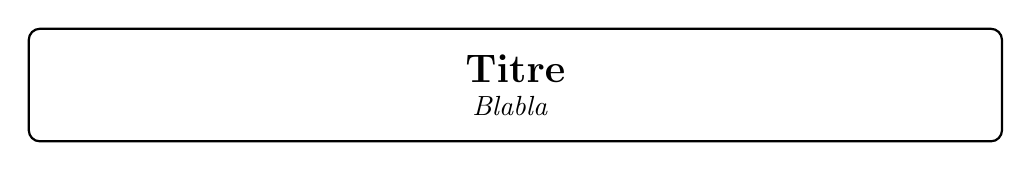
\begin{tikzpicture}
\node[rectangle,draw=black,rounded corners,thick,fill=white]{%
\begin{minipage}{\linewidth}
\begin{center}
\vspace*{6pt}
\textbf{\Large \bsc{Titre} }\par
\textit{Blabla}
\vspace*{6pt}
\end{center}
\end{minipage}
};\end{tikzpicture}


\noindent
\bigskip


\end{minipage}

\columnbreak

\begin{flushright}
\begin{minipage}{0.95\linewidth}
\textbf{TS$_1$} \hfill 2014-2015
\medskip

%cadre titre
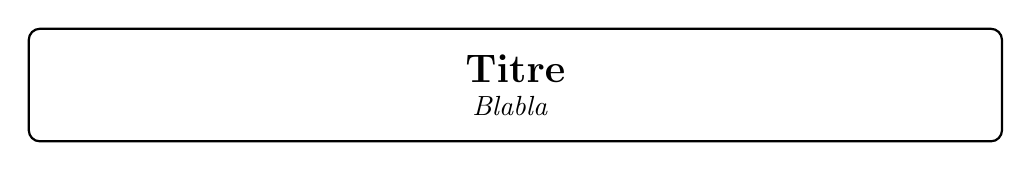
\begin{tikzpicture}
\node[rectangle,draw=black,rounded corners,thick,fill=white]{%
\begin{minipage}{\linewidth}
\begin{center}
\vspace*{6pt}
\textbf{\Large \bsc{Titre} }\par
\textit{Blabla}
\vspace*{6pt}
\end{center}
\end{minipage}
};\end{tikzpicture}


\noindent


\end{minipage}
\end{flushright}
\end{multicols}







%%%%%%%%%%%%%%%%%%%%%%%%%%%%%%%%%%%%%%%%%%%%%%%%

%





\end{document}
